


\begin{tabular}{c}

\begin{tabular}{ | c   p{18cm} |}
	\hline
	%\rowcolor{blue!30}
	\cellcolor{black}\rotcell{\large\textbf{\textcolor{white}{Allgemein}}}  &
	\setlength{\extrarowheight}{5pt}			
	\begin{tabular}{L{5cm} L{6.5cm} L{5.3cm}}
		\textbf{Arbeit, Energie}
		&$\Delta W=\int_{L} \mathbf{F} \cdot d \mathbf{l}=W_{1}-W_{2}$
		&$[\Delta W]=[W]=\mathrm{J}=\mathrm{W} \mathrm{s}$, \qquad $[F]=\mathrm{N}=\mathrm{kg} \cdot \mathrm{m} / \mathrm{s}^{2}$ \\[5pt]
		
		
		\rowcolor[rgb]{0.91,0.91,0.91}
		\textbf{Drehmoment} &
		$\mathbf{T}=\mathbf{r} \times \mathbf{F} \quad$ (T auf Drehachse)&
		$[T]=\mathrm{Nm}=\mathrm{kg} \cdot \mathrm{m}^2 / \mathrm{s}^{2},[r]=\mathrm{m}$\\[5pt]
		
		
		\rowcolor[rgb]{1,1,1}\textbf{Zentripedalkraft}&
		$\displaystyle \mathbf{F}=\frac{m v^{2}}{r}(-\hat{\mathbf{r}})=-m \omega^{2} \mathbf{r}$&
		$[m]=\mathrm{kg},[r]=\mathrm{m}$, \qquad	$[v]=m / s,[\omega]=\mathrm{rad} / s$		\\[5pt]
		
		\rowcolor[rgb]{0.91,0.91,0.91}
		\textbf{Lorenzkraft} &$\mathbf{F}_{L}=\mathbf{F}_{C}+\mathbf{F}_{A}=q(\mathbf{E}+\mathbf{v} \times \mathbf{B})$&
		$[E]=\mathrm{V} / \mathrm{m},[B]=\mathrm{A} / \mathrm{m}$   
		\qquad $[v]=\mathrm{m} / \mathrm{s},[l]=\mathrm{m}$ \\[5pt]
		
		
		\rowcolor[rgb]{1,1,1}\textbf{Drehimpuls}&
		$\boldsymbol{L}=\boldsymbol{r} \times \boldsymbol{p}$&
		$[L]=\mathrm{kg} \cdot \mathrm{m}^2 / \mathrm{s}$\\
		
		\rowcolor[rgb]{0.91,0.91,0.91}\textbf{Drallsatz}&$M=\dot{L}$ &\\
		
		
	\end{tabular}\\
	\hline
\end{tabular}\\

		\begin{tabular}{ | c   p{18cm} |}
			\hline
			\cellcolor{black}\rotcell{\large\textbf{\textcolor{white}{Wellen}}}  &
			\setlength{\extrarowheight}{10pt}			
			\begin{tabular}{L{5cm} L{7cm} L{5cm}}
				\textbf{Wellengleichung}
				 1 und 3 Dimensional &
				 $\displaystyle \frac{\partial^{2} \xi}{\partial t^{2}}-v^{2} \frac{\partial^{2} \xi}{\partial x^{2}}=0$ \qquad $\displaystyle\frac{\partial^{2} \vec{\xi}}{\partial t^{2}}-v^{2} \Delta \vec{\xi}=0$ &Allg. Lösung $\xi(x, t)=f(x \pm v t)$ \\[10pt]
				
				\rowcolor[rgb]{0.91,0.91,0.91}
				Harmonische Lösung: & 
				$\displaystyle \xi(x, t) =\xi_{0} \sin (k(x \pm v t))=\xi_{0} \sin (k x \pm \omega t) =\xi_{0} e^{i(k x \pm \omega t)}
				$ & 
				$-v$ rechtslaufend $+v$ linkslaufend \\[10pt]
				
				\rowcolor[rgb]{1,1,1}
				\textbf{Wellenlänge \& Wellenzahl}  &$\displaystyle \lambda=\frac{v}{f}=\frac{2\pi}{k}=v\cdot T$\qquad $\displaystyle k=|\mathbf{k}|=\omega \sqrt{\varepsilon \mu}=\frac{\omega}{v}=\frac{2 \pi}{\lambda}$ & $\left[\lambda\right]=\mathrm{m}$ $[k]=\mathrm{rad} / \mathrm{m}$\\[10pt]
				
				\rowcolor[rgb]{0.91,0.91,0.91}
				\textbf{Seilwelle} Transversal (Zugspannung $\mathrm{S}$) & $\displaystyle v^{2}=\frac{S}{\rho} \quad$ , $\displaystyle\quad S=\frac{F}{A\quad}$ , $\displaystyle \quad\rho=\frac{m}{V} \quad$&
				$\left[\mathrm{F}\right]=\mathrm{kg}\cdot\mathrm{m}/\mathrm{s} ^{2}$\qquad\qquad\qquad
				Dichte
				$\left[\mathrm{\rho}\right]=\mathrm{kg}/\mathrm{m}^{3}$ \\[5pt]
				
				
				\rowcolor[rgb]{1,1,1}
				\textbf{Festkörper} Longitudalwelle \quad ($E$ Elastizitätmodul)  & $\displaystyle v^{2}=\frac{E}{\rho} \quad$ , $\displaystyle\quad E=\sigma\frac{l}{\Delta l}$&
				$\left[\mathrm{E}\right]=\mathrm{N}/\mathrm{m}^{-2}$\qquad
				Normalspannung
				 $\left[\mathrm{\sigma}\right]=\frac{\mathrm{dF_{\bot}}}{da}\mathrm{N}/\mathrm{m}^{-2}$ \\[5pt]
				
				
				\rowcolor[rgb]{0.91,0.91,0.91}
				\textbf{Ebene Welle}  \qquad \qquad harmonische Welle  & $\displaystyle \vec{\xi}(x, y, z, t)=\vec{A} e^{i(\vec{k} \cdot \vec{r}-\omega t)}$&
				(Die zu $\vec{k}$ senkrechte Ebene ist $\vec{k} \cdot \vec{r}=$ konst. $)$\\[5pt]
				
				\rowcolor[rgb]{1,1,1}
				\textbf{Kugel Welle} \qquad \qquad harmonische Welle  & $\displaystyle \vec{\xi}(\vec{r}, t)=\frac{\overrightarrow{A_{1}}}{r} f_{1}(\vec{k} \cdot \vec{r}-w t)+\frac{\overrightarrow{A_{2}}}{r} f_{2}(\vec{k} \cdot \vec{r}+w t)$& $\displaystyle I = \frac{P}{4\pi r^2}$ Intensität $I$ \qquad Leistung $P$ über $r^2$
				\\
				
				\rowcolor[rgb]{1,1,1}
				\multicolumn{3}{l}{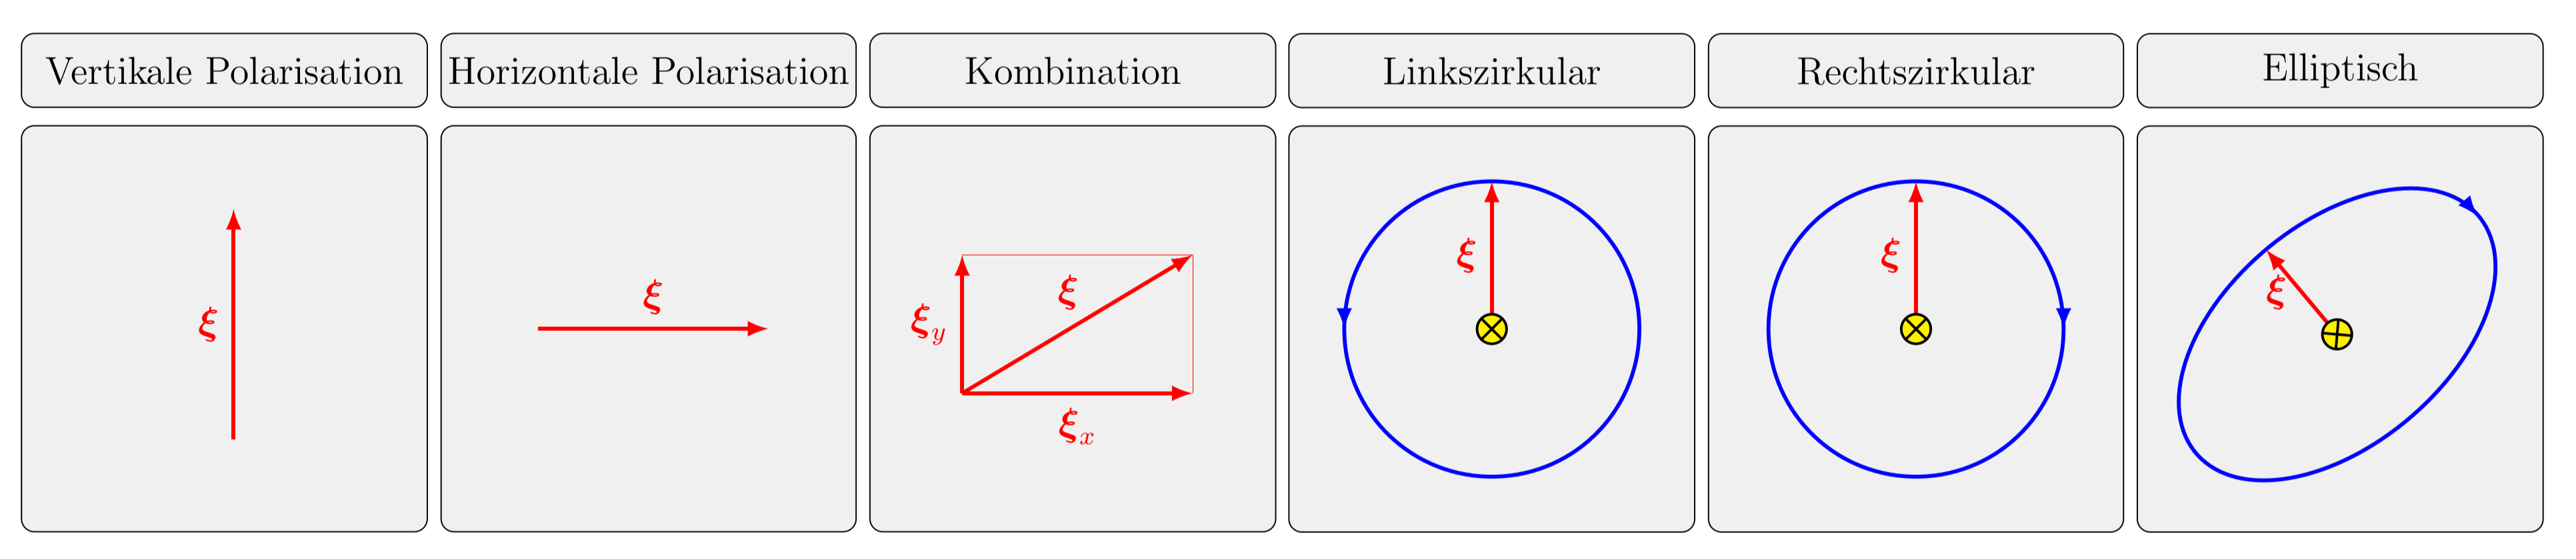
\includegraphics[width=17.8cm]{polarisation.png}}\\
	
			\rowcolor[rgb]{1,1,1}
			\textbf{Gesetzt von Malus} Polarisationsfilter & $\displaystyle I=I_{0} \cdot \cos ^{2}(\alpha)$ & $\alpha$ Polarisationswinkel \qquad\qquad\qquad $I_0$ Intensität \\[5pt]



			\rowcolor[rgb]{0.91,0.91,0.91}
			\textbf{Mittlere harmonische Energiedichte}  über Periode T  & $\displaystyle\left\langle\frac{\mathrm{d} W}{\mathrm{~d} V}\right\rangle=\frac{1}{T} \int_{0}^{T} \frac{\mathrm{d} W}{\mathrm{~d} V}(x, t) \mathrm{d} t=\frac{1}{2} \rho \omega^{2} A^{2}$&
			Energie pro Zeiteinheit und pro Flächeneinheit \\[10pt]
			
			\rowcolor[rgb]{1,1,1}
			\textbf{Mittlere Intensität} harmonische Welle  & $\displaystyle \langle I\rangle=\frac{1}{2} \rho \omega^{2} A^{2} v=\frac{1}{2} \rho \frac{\omega^{3}}{k} A^{2}= \frac{1}{2} \rho \sqrt{\frac{F}{\rho \pi R^{2}}} \omega^{2} A^{2} \propto \sqrt{\rho} A^{2}$&
			Energie pro Zeiteinheit und pro Flächeneinheit \\[20pt]
			
			\rowcolor[rgb]{0.91,0.91,0.91}
			\textbf{Poynting-Theorem}  Poynting-Vektor:   & $\displaystyle \mathbf{S}=\frac{\mathrm{d}^{2} W}{\mathrm{~d} a \mathrm{~d} t} \frac{\mathrm{d} \vec{a}}{|\mathrm{~d} \vec{a}|}$\qquad , \qquad
			$\displaystyle \mathbf{S}=\mathbf{E} \times \mathbf{H}$&$\displaystyle[S]=\frac{\mathrm{W}}{\mathrm{m}^{2}}$
			\\
			
			\rowcolor[rgb]{1,1,1}
			\textbf{Dopplereffekt} &
			$\displaystyle f_{B}=\frac{c+v_{b}}{c-v_{q}} f_{q}$  \qquad $c_{\text{Luft}}= 340m/s$ &
			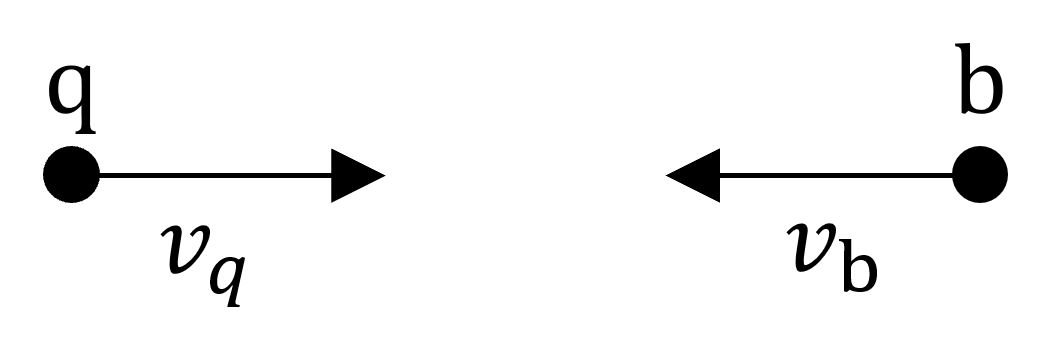
\includegraphics[width=3cm]{doppler.jpg} \\[5pt]
			
					\rowcolor[rgb]{0.91,0.91,0.91}
			\textbf{Schockwelle} & 
			$\displaystyle \vartheta=\arcsin \left(\frac{u}{v_{Q}}\right)$ & 
			$\displaystyle \vartheta$ Halber Öffnungswinkel Machscher Kegel \\[5pt]
			
			
	
			

		\end{tabular}\\[5pt]
		\hline
\end{tabular}
\end{tabular}
\begin{tabular}{ | c   p{18cm} |}
		\hline
		\cellcolor{black}\rotcell{\large\textbf{\textcolor{white}{Wellen}}}  &
		\setlength{\extrarowheight}{10pt}			
		\begin{tabular}{L{5cm} L{7cm} L{5cm}}

				
				&$\displaystyle -\frac{d}{d t} \int_{V}\left(w_{e}+w_{m}\right) d v=\int_{V} p d v+\int_{A=\partial V} \mathbf{S} \cdot d \mathbf{s}$&  $I:=|\vec{S}|$ (Intsensität) \\[10pt]
				
				\rowcolor[rgb]{1,1,1}
				\textbf{Beispiel}  Poyting Vector Ohmischer-Widerstand   &$\displaystyle|\mathbf{S}|=|\mathbf{E} \times \mathbf{H}|=\frac{U \cdot I}{2 \pi R l}$ Integral Mantelfläche
				$\displaystyle P=\oint_{M} \vec{S} \cdot \mathrm{d} \vec{A}=-\frac{U \cdot I}{2 \pi R l} \cdot 2 \pi R l=-U \cdot I$  & elt. Feldstärke $\displaystyle |\vec{E}|=\frac{U}{l}$ ,\qquad mag. Feldstärke$|\displaystyle\vec{H}|=\frac{I}{2 \pi R}$ \\[20pt]

			
			\rowcolor[rgb]{0.91,0.91,0.91}
			\textbf{Energietransport} \qquad kinetische Energiedichte   & $\displaystyle \frac{\mathrm{d} T}{\mathrm{~d} V}=\frac{1}{2} \rho\left(\frac{\partial \xi}{\partial t}\right)^{2}=\frac{1}{2} \rho v^{2}\left(\frac{\mathrm{d} \xi}{\mathrm{d}(x-v t)}\right)^{2}$& Energie $\mathrm{d} T$ \qquad gilt nur für mechanische Wellen
			\\
			elastische Energiedichte & $\displaystyle \frac{\mathrm{d} E_{e l}}{\mathrm{~d} V}=\frac{1}{2} E\left(\frac{\partial \xi}{\partial x}\right)^{2}=\frac{1}{2} S\left(\frac{\partial \xi}{\partial x}\right)^{2}=\frac{\mathrm{d} T}{\mathrm{~d} V}$& Bei Superposition Energien nicht addieren!\\[5pt]
				
			Gesamtenergiedichte &$\displaystyle \frac{\mathrm{d} W}{\mathrm{~d} V}=\frac{\mathrm{d} T}{\mathrm{~d} V}+\frac{\mathrm{d} E_{e l}}{\mathrm{~d} V}=\rho v^{2}\left(\frac{\mathrm{d} \xi}{\mathrm{d}(x-v t)}\right)^{2}=\rho v^{2} f^{\prime 2}$& $\xi(x, t)=f(u)$ mit  $u=x-v t$\qquad $\displaystyle f^{\prime 2}=\frac{\partial f}{\partial u}$ \\	[20pt]
			
			
			\rowcolor[rgb]{1,1,1}
			&&\\[-15pt]
			\textbf{Superposition} \qquad \qquad Harmonische Wellen &
			\multicolumn{2}{l}{\parbox{8cm}{$\displaystyle \xi=\underbrace{A \sin (k x-\omega t)}_{\xi_{1}(x, t)}+\underbrace{A \sin (k(x+\Delta x)-\omega t+\delta)}_{\xi_{2}(x, t)}= \underbrace{2 A \cos \left(\frac{1}{2}(\delta+k \Delta x)\right)}_{\text {Amplitude }} \underbrace{\sin \left(k x-\omega t+\frac{1}{2}(\delta+k \Delta x)\right)}_{\text {harmonische Welle }}$ }  } \\[10pt]
			
			Kontruktive/Destruktive Interferenz&$\frac{1}{2}(\delta+k \Delta x)=n \pi$ \quad $\frac{1}{2}(\delta+k \Delta x)=\left(n+\frac{1}{2}\right) \pi$& \\
			
			\rowcolor[rgb]{0.91,0.91,0.91}
			\textbf{Reflexion/Transmission} Auftreffend Welle& $\displaystyle\xi_{A}=A e^{i\left(k_{1} x-\omega t\right)}$ \qquad\qquad \qquad Transversal&  $\displaystyle k_{2}=\omega \sqrt{\frac{\rho_{2}}{S_{2}}}$, $ \displaystyle \alpha=\sqrt{\frac{S_{2} \rho_{2}}{S_{1} \rho_{1}}}$\\
			Reflektierte Welle&	$\displaystyle\xi_{R}=R e^{i\left(-k_{1} x-\omega t+\delta_{R}\right)}$ \qquad\qquad Longitudinal& $\displaystyle k_{2}=\omega \sqrt{\frac{\rho_{2}}{E_{2}}}$,$\displaystyle \alpha=\sqrt{\frac{E_{2} \rho_{2}}{E_{1} \rho_{1}}}$ \\
			Transmitierte Welle&$\displaystyle \xi_{T}=T e^{i\left(k_{2} x-\omega t+\delta_{T}\right)}$&  gesucht: $\displaystyle R,T,\delta_{R}, \delta_{T}, k_{2} $ \\
			Phase &$\delta_{R}=0 \qquad \delta_{R}=\pi \qquad \delta_{T}=0$&\\
			Amplitude &$R=\frac{1-\alpha}{1+\alpha} A \quad R=-\frac{1-\alpha}{1+\alpha} A$\qquad $T=\frac{2 A}{1+\alpha}$&$(R \geq 0)$ \\
			
			
			\textbf{Spezialfall} \qquad festes (Seil-)Ende $(\alpha \rightarrow \infty)$& $\displaystyle\underbrace{\delta R=\pi}_{\pi \text { Phasensprung }}$\quad$\displaystyle\lim _{\alpha \rightarrow \infty} R=A$\quad $\displaystyle \lim _{\alpha \rightarrow \infty} T=0$ &($\alpha = 0$ nur bei übergang zu Vakuum. mech. Welle
			kann nicht ins Vakuum, d.h $T = 0$ statt $T = 2A$)\\
			loses (Seil-) Ende $(\alpha \rightarrow 0)$&$\displaystyle\underbrace{\delta R=0}_{\text {kein Phasensprung }}$ , $\displaystyle \lim _{\alpha \rightarrow \infty} R=A$, $\displaystyle\lim _{\alpha \rightarrow \infty} T=0$&\\[10pt]
			
			&&\\[-15pt]
			\rowcolor[rgb]{1,1,1}
			\textbf{Snellius’sche Brechungsgesetz} &
			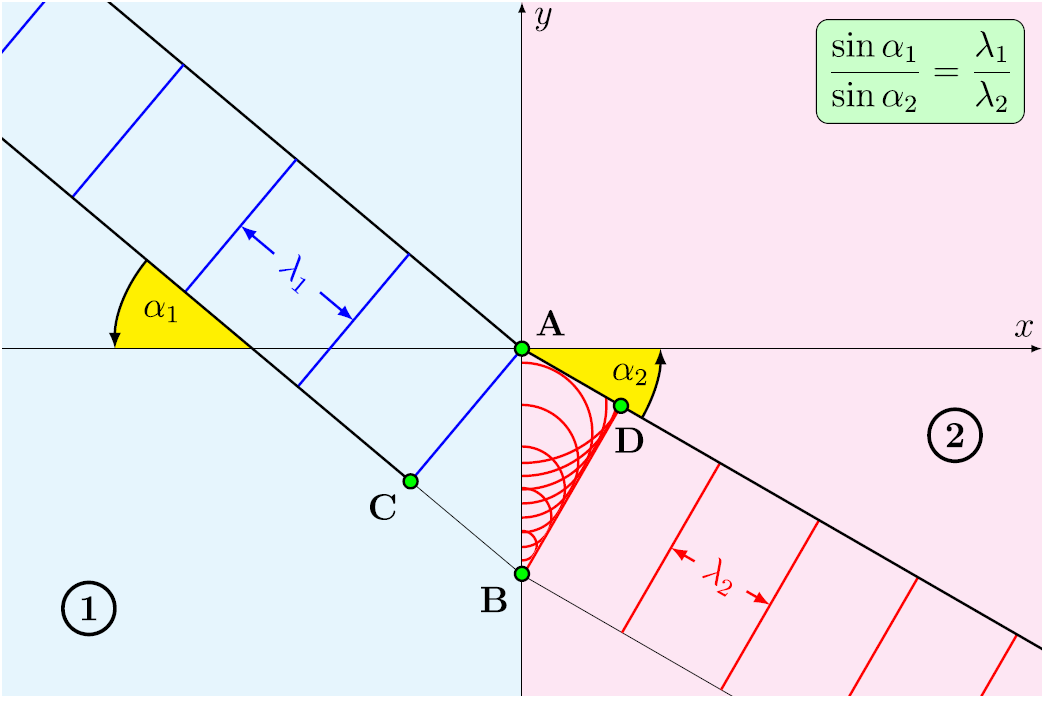
\includegraphics[width=7cm]{huygens2.png}&$\displaystyle\frac{\sin \left(\alpha_{1}\right)}{\sin \left(\alpha_{2}\right)}=\frac{v_{1}}{v_{2}}=\frac{\lambda_{1}}{\lambda_{2}}$ \\[10pt]
			
			
			\rowcolor[rgb]{0.91,0.91,0.91}
			&&\\[-15pt]
			\textbf{Fermat’sches Prinzip}&\multicolumn{2}{l}{\parbox{12cm}{Nach dem Fermat’schen Prinzip läuft eine Welle bei Reflexion und Brechung, stets jenen Weg, für den die Laufzeit einer Phasenfläche $\Phi$ zwischen zwei Punkten minimal wird.}}
			\\[20pt]
			
				
			\end{tabular}\\[5pt]
			\hline
		\end{tabular}
	
	
	\begin{tabular}{ | c   p{18cm} |}
	\hline
	\cellcolor{black}\rotcell{\large\textbf{\textcolor{white}{Wellen}}}  &
	\setlength{\extrarowheight}{10pt}			
	\begin{tabular}{L{5cm} L{7cm} L{5cm}}
		
		
	
		
	
		\rowcolor[rgb]{1,1,1}
		&&\\[-15pt]	
		\textbf{Stehende Wellen} \qquad \qquad gegeenlaufende Harmonische Wellen &
		\multicolumn{2}{l}{\parbox{8cm}{$\displaystyle \xi(x,t)=\underbrace{A \sin (k x-\omega t)}_{\xi_{1}(x, t)}+\underbrace{A \sin (kx+\omega t+\delta)}_{\xi_{2}(x, t)}= \underbrace{2 A \sin \left(kx+\frac{\delta}{2}\right)}_{\text {Amplitude }} \underbrace{\cos \left(\omega t+\frac{\delta}{2}\right)}_{\text {harmonische Welle }}$ }  } \\[10pt]
		
		Saite fest-fest ($n$-te Normalschwingung) &$\xi_{n}(x, t)=A_{n} \sin \left(\frac{n \pi}{l} x\right) \cos \left(\frac{n \pi}{l} v t+\varphi_{n}\right)$&\\
		Saite fest-offen&$\displaystyle\xi_{n}(x, t)=A_{n} \sin \left(\frac{2 n+1}{2} \frac{\pi}{l} x\right) \cos \left(\frac{2 n+1}{2} \frac{\pi}{l} v t+\varphi_{n}\right)$&\\
		
		
		
		\rowcolor[rgb]{0.91,0.91,0.91}
		&&\\[-15pt]
		\textbf{Prinzip von Huygens}&\multicolumn{2}{l}{\parbox{12cm}{Jeder Punkt einer bestehenden Wellenfläche (bzw. Wellenfront) wird als Zentrum einer neuen kugelförmigen Elementarwelle aufgefasst. Die Umhüllende dieser Elementarwellen ergibt dann die Wellenfront zu einem späteren Zeitpunkt.}}
		\\[20pt]
		
		\rowcolor[rgb]{1,1,1}
		\textbf{Einzelspalt} &
		$\displaystyle\langle I\rangle \propto A^{2} \frac{\sin ^{2}\left(\frac{\Delta \varphi}{2}\right)}{\left(\frac{\Delta \varphi}{2}\right)^{2}}$
		mit $\quad \Delta \varphi=k d \sin (\alpha)$ &$\Delta \varphi$ Phasendifferenz	 \\[10pt]
		
		
		\textbf{Beispiel}&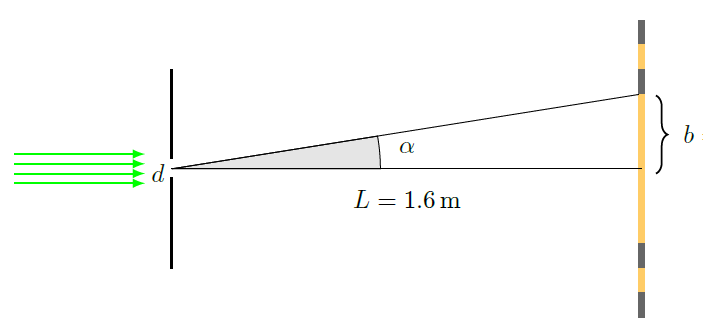
\includegraphics[width=7cm]{spalt.png}& $\langle I\rangle \sim A^{2} \frac{\sin ^{2}\left(\frac{1}{2} \Delta \varphi\right)}{\left(\frac{1}{2} \Delta \varphi\right)^{2}}, \quad$ mit $\quad \Delta \varphi=2 \pi \frac{d}{\lambda} \sin \alpha$ $I$ verschwindet bei $\frac{1}{2} \Delta \varphi=n \pi, n \in \mathbb{N}$ \qquad $\Rightarrow d=n \frac{\lambda}{\sin \alpha}=n \frac{\lambda}{b/L}$\\
		
		
	
		
	\end{tabular}\\[5pt]
	\hline
\end{tabular}	
	
	

	
